\centering
\begin{minipage}{0.24\linewidth}\centering
  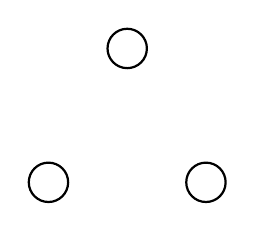
\begin{tikzpicture}[auto,
    specification/.style ={circle, draw, thick,inner sep=0pt, minimum size=5mm}]
   \node[specification] (A)  at (-1,0)  {};
   \node[specification] (B)  at (1,0)  {};
   \node[specification] (C)  at (0,1.7)  {};
 \end{tikzpicture}\\
  \vspace*{0.3cm}
  A
\end{minipage}\hfill
\begin{minipage}{0.24\linewidth}\centering
  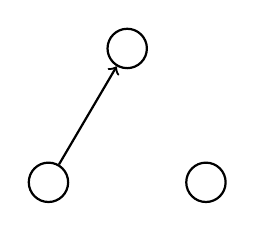
\begin{tikzpicture}[auto,
    specification/.style ={circle, draw, thick,inner sep=0pt, minimum size=5mm}]
   \node[specification] (A)  at (-1,0)  {};
   \node[specification] (B)  at (1,0)  {};
   \node[specification] (C)  at (0,1.7)  {};
   \draw[thick, ->] (A) to  (C);
 \end{tikzpicture}\\
   \vspace*{0.3cm}
B
\end{minipage}\hfill
 \begin{minipage}{0.24\linewidth}\centering
  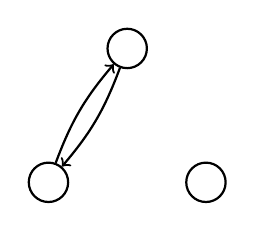
\begin{tikzpicture}[auto,
    specification/.style ={circle, draw, thick,inner sep=0pt, minimum size=5mm}]
   \node[specification] (A)  at (-1,0)  {};
   \node[specification] (B)  at (1,0)  {};
   \node[specification] (C)  at (0,1.7)  {};
   \draw[thick, ->] (A) to  [bend left=10] (C);
   \draw[thick, ->] (C) to  [bend left=10] (A);   
 \end{tikzpicture}\\
   \vspace*{0.3cm}
C
\end{minipage}\hfill
 \begin{minipage}{0.24\linewidth}\centering
  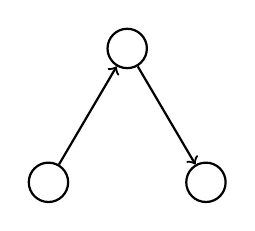
\begin{tikzpicture}[auto,
    specification/.style ={circle, draw, thick,inner sep=0pt, minimum size=5mm}]
   \node[specification] (A)  at (-1,0)  {};
   \node[specification] (B)  at (1,0)  {};
   \node[specification] (C)  at (0,1.7)  {};
   \draw[thick, ->] (A) to  (C);
   \draw[thick, ->] (C) to  (B);
 \end{tikzpicture}\\
   \vspace*{0.3cm}
D
\end{minipage}

\vspace{0.3cm}
 \begin{minipage}{0.24\linewidth}\centering
  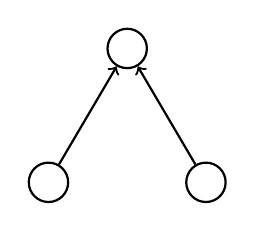
\begin{tikzpicture}[auto,
    specification/.style ={circle, draw, thick,inner sep=0pt, minimum size=5mm}]
   \node[specification] (A)  at (-1,0)  {};
   \node[specification] (B)  at (1,0)  {};
   \node[specification] (C)  at (0,1.7)  {};
   \draw[thick, ->] (A) to  (C);
   \draw[thick, ->] (B) to  (C);
\end{tikzpicture}\\
  \vspace*{0.3cm}
  E
\end{minipage}\hfill
 \begin{minipage}{0.24\linewidth}\centering
  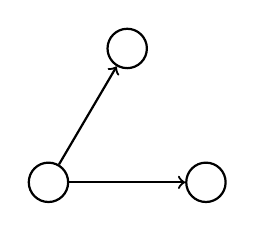
\begin{tikzpicture}[auto,
    specification/.style ={circle, draw, thick,inner sep=0pt, minimum size=5mm}]
   \node[specification] (A)  at (-1,0)  {};
   \node[specification] (B)  at (1,0)  {};
   \node[specification] (C)  at (0,1.7)  {};
   \draw[thick, ->] (A) to  (C);
   \draw[thick, ->] (A) to  (B);
\end{tikzpicture}\\
  \vspace*{0.3cm}
  F
\end{minipage}\hfill
 \begin{minipage}{0.24\linewidth}\centering
  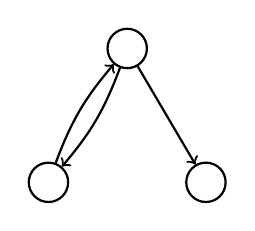
\begin{tikzpicture}[auto,
    specification/.style ={circle, draw, thick,inner sep=0pt, minimum size=5mm}]
   \node[specification] (A)  at (-1,0)  {};
   \node[specification] (B)  at (1,0)  {};
   \node[specification] (C)  at (0,1.7)  {};
   \draw[thick, ->] (A) to  [bend left=10] (C);
   \draw[thick, ->] (C) to  [bend left=10] (A);
   \draw[thick, ->] (C) to  (B);   
\end{tikzpicture}\\
  \vspace*{0.3cm}
  G
\end{minipage}\hfill
 \begin{minipage}{0.24\linewidth}\centering
  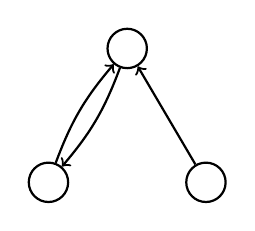
\begin{tikzpicture}[auto,
    specification/.style ={circle, draw, thick,inner sep=0pt, minimum size=5mm}]
   \node[specification] (A)  at (-1,0)  {};
   \node[specification] (B)  at (1,0)  {};
   \node[specification] (C)  at (0,1.7)  {};
   \draw[thick, ->] (A) to  [bend left=10] (C);
   \draw[thick, ->] (C) to  [bend left=10] (A);
   \draw[thick, ->] (B) to  (C);
 \end{tikzpicture}\\
  \vspace*{0.3cm}
  H
\end{minipage}

\vspace{0.3cm}
 \begin{minipage}{0.24\linewidth}\centering
  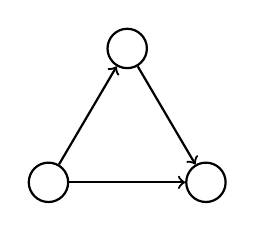
\begin{tikzpicture}[auto,
    specification/.style ={circle, draw, thick,inner sep=0pt, minimum size=5mm}]
   \node[specification] (A)  at (-1,0)  {};
   \node[specification] (B)  at (1,0)  {};
   \node[specification] (C)  at (0,1.7)  {};
   \draw[thick, ->] (A) to  (C);
   \draw[thick, ->] (C) to  (B);
   \draw[thick, ->] (A) to  (B);   
\end{tikzpicture}\\
  \vspace*{0.3cm}
  I
\end{minipage}\hfill
 \begin{minipage}{0.24\linewidth}\centering
  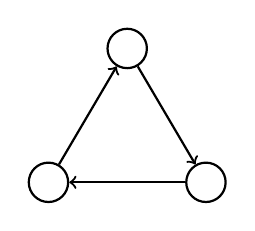
\begin{tikzpicture}[auto,
    specification/.style ={circle, draw, thick,inner sep=0pt, minimum size=5mm}]
   \node[specification] (A)  at (-1,0)  {};
   \node[specification] (B)  at (1,0)  {};
   \node[specification] (C)  at (0,1.7)  {};
   \draw[thick, ->] (A) to  (C);
   \draw[thick, ->] (C) to  (B);
   \draw[thick, ->] (B) to  (A);
 \end{tikzpicture}\\
  \vspace*{0.3cm}
  J
\end{minipage}\hfill
 \begin{minipage}{0.24\linewidth}\centering
  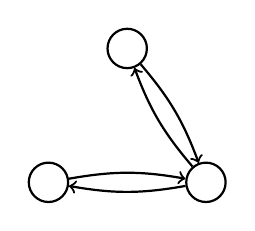
\begin{tikzpicture}[auto,
    specification/.style ={circle, draw, thick,inner sep=0pt, minimum size=5mm}]
   \node[specification] (A)  at (-1,0)  {};
   \node[specification] (B)  at (1,0)  {};
   \node[specification] (C)  at (0,1.7)  {};
   \draw[thick, ->] (A) to  [bend left=10] (B);
   \draw[thick, ->] (B) to  [bend left=10] (A);
   \draw[thick, ->] (B) to  [bend left=10] (C);
   \draw[thick, ->] (C) to  [bend left=10] (B);
 \end{tikzpicture}\\
  \vspace*{0.3cm}
  K
\end{minipage}\hfill
 \begin{minipage}{0.24\linewidth}\centering
  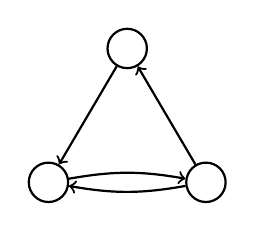
\begin{tikzpicture}[auto,
    specification/.style ={circle, draw, thick,inner sep=0pt, minimum size=5mm}]
   \node[specification] (A)  at (-1,0)  {};
   \node[specification] (B)  at (1,0)  {};
   \node[specification] (C)  at (0,1.7)  {};
   \draw[thick, ->] (A) to  [bend left=10] (B);
   \draw[thick, ->] (B) to  [bend left=10] (A);
   \draw[thick, ->] (B) to  (C);
   \draw[thick, ->] (C) to  (A);
 \end{tikzpicture}\\
  \vspace*{0.3cm}
  L
\end{minipage}

\vspace{0.3cm}
 \begin{minipage}{0.24\linewidth}\centering
   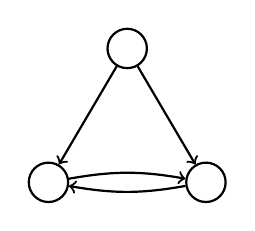
\begin{tikzpicture}[auto,
    specification/.style ={circle, draw, thick,inner sep=0pt, minimum size=5mm}]
   \node[specification] (A)  at (-1,0)  {};
   \node[specification] (B)  at (1,0)  {};
   \node[specification] (C)  at (0,1.7)  {};
   \draw[thick, ->] (A) to  [bend left=10] (B);
   \draw[thick, ->] (B) to  [bend left=10] (A);
   \draw[thick, ->] (C) to  (B);
   \draw[thick, ->] (C) to  (A);
 \end{tikzpicture}\\
  \vspace*{0.3cm}
  M
\end{minipage}\hfill
 \begin{minipage}{0.24\linewidth}\centering
  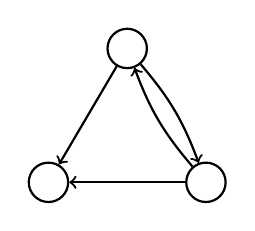
\begin{tikzpicture}[auto,
    specification/.style ={circle, draw, thick,inner sep=0pt, minimum size=5mm}]
   \node[specification] (A)  at (-1,0)  {};
   \node[specification] (B)  at (1,0)  {};
   \node[specification] (C)  at (0,1.7)  {};
   \draw[thick, ->] (C) to   (A);
   \draw[thick, ->] (B) to   (A);
   \draw[thick, ->] (B) to  [bend left=10] (C);
   \draw[thick, ->] (C) to  [bend left=10] (B);
 \end{tikzpicture}\\
  \vspace*{0.3cm}
  N
\end{minipage}\hfill
 \begin{minipage}{0.24\linewidth}\centering
  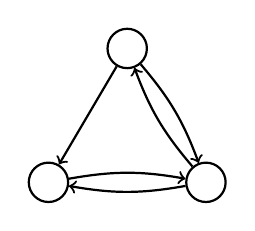
\begin{tikzpicture}[auto,
    specification/.style ={circle, draw, thick,inner sep=0pt, minimum size=5mm}]
   \node[specification] (A)  at (-1,0)  {};
   \node[specification] (B)  at (1,0)  {};
   \node[specification] (C)  at (0,1.7)  {};
   \draw[thick, ->] (A) to  [bend left=10] (B);
   \draw[thick, ->] (B) to  [bend left=10] (A);
   \draw[thick, ->] (B) to  [bend left=10] (C);
   \draw[thick, ->] (C) to  [bend left=10] (B);
   \draw[thick, ->] (C) to   (A);   
 \end{tikzpicture}\\
  \vspace*{0.3cm}
  O
\end{minipage}\hfill
 \begin{minipage}{0.24\linewidth}\centering
  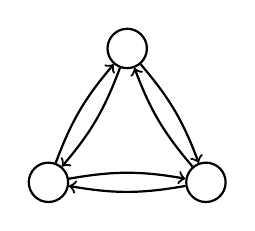
\begin{tikzpicture}[auto,
    specification/.style ={circle, draw, thick,inner sep=0pt, minimum size=5mm}]
   \node[specification] (A)  at (-1,0)  {};
   \node[specification] (B)  at (1,0)  {};
   \node[specification] (C)  at (0,1.7)  {};
   \draw[thick, ->] (A) to  [bend left=10] (B);
   \draw[thick, ->] (B) to  [bend left=10] (A);
   \draw[thick, ->] (B) to  [bend left=10] (C);
   \draw[thick, ->] (C) to  [bend left=10] (B);
   \draw[thick, ->] (A) to  [bend left=10] (C);
   \draw[thick, ->] (C) to  [bend left=10] (A);   
 \end{tikzpicture}\\
  \vspace*{0.3cm}
  P
\end{minipage}
